\documentclass[smaller]{beamer}\usepackage[]{graphicx}\usepackage[]{color}
% maxwidth is the original width if it is less than linewidth
% otherwise use linewidth (to make sure the graphics do not exceed the margin)
\makeatletter
\def\maxwidth{ %
  \ifdim\Gin@nat@width>\linewidth
    \linewidth
  \else
    \Gin@nat@width
  \fi
}
\makeatother

\definecolor{fgcolor}{rgb}{0.345, 0.345, 0.345}
\newcommand{\hlnum}[1]{\textcolor[rgb]{0.686,0.059,0.569}{#1}}%
\newcommand{\hlstr}[1]{\textcolor[rgb]{0.192,0.494,0.8}{#1}}%
\newcommand{\hlcom}[1]{\textcolor[rgb]{0.678,0.584,0.686}{\textit{#1}}}%
\newcommand{\hlopt}[1]{\textcolor[rgb]{0,0,0}{#1}}%
\newcommand{\hlstd}[1]{\textcolor[rgb]{0.345,0.345,0.345}{#1}}%
\newcommand{\hlkwa}[1]{\textcolor[rgb]{0.161,0.373,0.58}{\textbf{#1}}}%
\newcommand{\hlkwb}[1]{\textcolor[rgb]{0.69,0.353,0.396}{#1}}%
\newcommand{\hlkwc}[1]{\textcolor[rgb]{0.333,0.667,0.333}{#1}}%
\newcommand{\hlkwd}[1]{\textcolor[rgb]{0.737,0.353,0.396}{\textbf{#1}}}%
\let\hlipl\hlkwb

\usepackage{framed}
\makeatletter
\newenvironment{kframe}{%
 \def\at@end@of@kframe{}%
 \ifinner\ifhmode%
  \def\at@end@of@kframe{\end{minipage}}%
  \begin{minipage}{\columnwidth}%
 \fi\fi%
 \def\FrameCommand##1{\hskip\@totalleftmargin \hskip-\fboxsep
 \colorbox{shadecolor}{##1}\hskip-\fboxsep
     % There is no \\@totalrightmargin, so:
     \hskip-\linewidth \hskip-\@totalleftmargin \hskip\columnwidth}%
 \MakeFramed {\advance\hsize-\width
   \@totalleftmargin\z@ \linewidth\hsize
   \@setminipage}}%
 {\par\unskip\endMakeFramed%
 \at@end@of@kframe}
\makeatother

\definecolor{shadecolor}{rgb}{.97, .97, .97}
\definecolor{messagecolor}{rgb}{0, 0, 0}
\definecolor{warningcolor}{rgb}{1, 0, 1}
\definecolor{errorcolor}{rgb}{1, 0, 0}
\newenvironment{knitrout}{}{} % an empty environment to be redefined in TeX

\usepackage{alltt}
\usepackage{amssymb}
\usepackage{amsmath}
\usepackage{graphicx}
\usepackage{hyperref}
\usepackage{multimedia}
\usepackage{epstopdf}
\usepackage{color}


\setcounter{MaxMatrixCols}{10}
\newtheorem{remark}{Remark}[section]
\newtheorem{proposition}{Proposition}[section]
\newtheorem{interpretation}{Interpretation}[section]
\newtheorem{goal}{Goal}[section]
\newtheorem{statement}{Statement}[section]
\newtheorem{aes}{Aim \& Scope}[section]
\newtheorem{exercise}{Exercise}[section]
\renewcommand{\Pr}{P}

\newcommand{\mbf}[1]{\mathbf{#1}}
\newcommand{\beq}{\begin{equation}}
\newcommand{\eeq}{\end{equation}}
\newcommand{\bea}{\begin{eqnarray}}
\newcommand{\eea}{\end{eqnarray}}
\newcommand{\ba}{\begin{array}}
\newcommand{\ea}{\end{array}}
\newcommand{\bi}{\begin{itemize}}
\newcommand{\ei}{\end{itemize}}
\newcommand{\ben}{\begin{enumerate}}
\newcommand{\een}{\end{enumerate}}
\newcommand{\nn}{\nonumber}

\newenvironment{stepenumerate}{\begin{enumerate}[<+->]}{\end{enumerate}}
\newenvironment{stepitemize}{\begin{itemize}[<+->]}{\end{itemize} }
\newenvironment{stepenumeratewithalert}{\begin{enumerate}[<+-| alert@+>]}{\end{enumerate}}
\newenvironment{stepitemizewithalert}{\begin{itemize}[<+-| alert@+>]}{\end{itemize} }
\usetheme{Madrid}


\definecolor{Mygreen}{rgb}{0.0,0.5,0.0}

%%%%%%%%%%%%%%%%%%%%%%%%%%%%%%%%%%%%%%%%%%%%%%%%%%%%%%%%%%%%%%%%%%%%%%%%%%%%%%%
% GSEM COLORS
%%%%%%%%%%%%%%%%%%%%%%%%%%%%%%%%%%%%%%%%%%%%%%%%%%%%%%%%%%%%%%%%%%%%%%%%%%%%%%%
\definecolor{darkGSEM}{RGB}{70,95,127}
\definecolor{darkGSEM2}{RGB}{40,80,150}
\definecolor{GSEM}{RGB}{96,121,153} % GSEM 10% lighter

%%% Global colors
\setbeamercolor*{palette primary}{use=structure,fg=white,bg=darkGSEM}
\setbeamercolor*{palette quaternary}{use=structure,fg=white,bg=darkGSEM!90}
\setbeamercolor{frametitle}{fg=white,bg=GSEM!80}

%%% TOC colors
\setbeamercolor{section in toc}{fg=darkGSEM}

%%% itemize colors
\setbeamertemplate{itemize items}[circle]
\setbeamercolor{itemize item}{fg=darkGSEM2}
\setbeamercolor{itemize subitem}{fg=darkGSEM2}
\setbeamercolor{itemize subsubitem}{fg=darkGSEM2}


%%% enumerate colors
\setbeamercolor{item projected}{fg=white,bg=GSEM}
\setbeamertemplate{enumerate item}{\insertenumlabel.}
\setbeamercolor{enumerate item}{fg=darkGSEM2}
\setbeamercolor{enumerate subitem}{fg=darkGSEM2}
\setbeamercolor{enumerate subsubitem}{fg=darkGSEM2}


\AtBeginSection[]
{
  \begin{frame}{\secname}
    %\frametitle{Outline}
    \tableofcontents[currentsection]
  \end{frame}
}

%%%%%%%%%%%%%%%%%%%%%%%%%%%%%%%%%%%%%%%%%%%%%%%%%%%%%%%%%%%%%%%%%%%%%%%%%%%%%%%%



\IfFileExists{upquote.sty}{\usepackage{upquote}}{}
\begin{document}

\title[S110015]{Probability 1}
\subtitle{Lecture 4: Discrete Random Variables - Part 2}
\author[Flores-Agreda, La Vecchia]{Dr. Daniel Flores-Agreda, \\[0.5em] \tiny{(based on the notes of Prof. Davide La Vecchia)}}
\date{Spring Semester 2021}

\begin{frame}
\titlepage
\end{frame}

\begin{frame}{Objectives}
  \begin{itemize}
  \item Describe some important discrete distributions
  \bigskip
  \begin{itemize}
  \item PMF, PDF, Expectation, Variance.
  \bigskip
  \item Illustrate case uses.
  \end{itemize}
  \end{itemize}
\end{frame}

\begin{frame}{Outline}
\framesubtitle{Some important Discrete Distributions}
  \tableofcontents
\end{frame}


\begin{frame}{Introduction}
  \begin{remark}
  Their main common characteristic is that the probability $P\left(\left\{ X=x_i\right\}\right)$ is given by an appropriate mathematical formula: i.e.
  $$
  p_{i}=P\left(\left\{ X=x_i\right\}\right)=h(x_{i})
  $$
  for a suitably specified function $h(\cdot)$.
  \end{remark}
\end{frame}

%%%%%%%%%%%%%%%%%%%%%%%%%%%%%%%%%%%%%%%%%%%%%%%%%%%%%%%%
\section{Discrete Uniform}
%%%%%%%%%%%%%%%%%%%%%%%%%%%%%%%%%%%%%%%%%%%%%%%%%%%%%%%%

\begin{frame}{\secname}
  \begin{small}
  \begin{definition}
  We say $X$ has a \textbf{discrete uniform distribution} when

  \begin{itemize}
  \item $X$ can take the values $x=0,1,2,...,k$ (for some specified finite value $k\in \mathbb{N}$)
  \item The probability that $X=x$ is $1/\left( k+1\right) $ is given by the \textbf{PMF}:
  $$
  P\left(\left\{ X=x\right\}\right) = \frac{1}{\left( k+1\right)}.
  $$

  \pause
  \item The probability \textbf{distribution} is given by
  \begin{small}
  \begin{equation*}
  \begin{tabular}{|c|c|}
  \hline
  $x_i$ & $P \left(\left\{ X=x_i\right\}\right) $ \\ \hline\hline
  $0$ & $\frac{1}{\left( k+1\right) }$ \\ \hline
  $1$ & $\frac{1}{\left( k+1\right) }$ \\ \hline
  $\vdots $ & $\vdots $ \\ \hline
  $k$ & $\frac{1}{\left( k+1\right) }$ \\ \hline\hline
  Total & $1$ \\ \hline
  \end{tabular}
  \end{equation*}
  \end{small}
  \end{itemize}
  \end{definition}
  \end{small}
\end{frame}

\begin{frame}{\secname}
\framesubtitle{Expectation}
  \begin{stepitemize}
  \item The \textbf{Expectation} of $X$ is
  \begin{eqnarray*}
  E\left[ X\right] &=&  x_1 p_1 + ... +  x_k p_k\\
  &=& 0\cdot \frac{1}{\left( k+1\right) }+1\cdot \frac{1}{
  \left( k+1\right) }+\cdots +k\cdot \frac{1}{\left( k+1\right) } \\
  &=&\frac{1}{\left( k+1\right) }\cdot\left( 0+1+\cdots +k\right) \\
  &=&\frac{1}{\left( k+1\right) }\cdot \frac{k\left( k+1\right) }{2} \\
  &=&\frac{k}{2}.
  \end{eqnarray*}

  \begin{example}
  \begin{footnotesize}
  Consider $k=6$, then $X$ can take on one of the seven distinct values
  $x=0,1,2,3,4,5,6,$ each with equal probability $\frac{1}{7}$, and $E(X)=3$ (which is one of the possible outcomes).
  \end{footnotesize}
  \end{example}
  \end{stepitemize}
\end{frame}

\begin{frame}{\secname}
\framesubtitle{Variance and Standard Deviation}
  \begin{stepitemize}
  \item The variance of $X$ is:
  \begin{eqnarray*}
  Var\left( X\right) &=&\left( 0-\frac{k}{2}\right) ^{2}\cdot \frac{1}{\left(
  k+1\right) }+\left( 1-\frac{k}{2}\right) ^{2}\cdot \frac{1}{\left(
  k+1\right) }+ \\
  &&\cdots +\left( k-\frac{k}{2}\right) ^{2}\cdot \frac{1}{\left( k+1\right) }
  \\
  &=&\frac{1}{\left( k+1\right) }\cdot\left\{ \left( 0-\frac{k}{2}\right)
  ^{2}+\left( 1-\frac{k}{2}\right) ^{2}+\cdots +\left( k-\frac{k}{2}\right)
  ^{2}\right\} \\
  &=&\frac{1}{\left( k+1\right) }\cdot \frac{k\left( k+1\right) \left(
  k+2\right) }{12} \\
  &=&\frac{k\left( k+2\right) }{12}
  \end{eqnarray*}

  \begin{example}
  \begin{footnotesize}
  When $k=6$, then  $Var(X) = 4$ and $s.d(X)= \sqrt{4}=2$.
  \end{footnotesize}
  \end{example}
  \end{stepitemize}
\end{frame}

\begin{frame}{\secname}%
\framesubtitle{Illustrations}
  \begin{figure}[ptb]\centering
  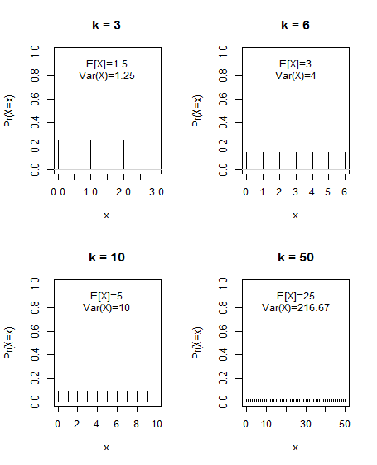
\includegraphics[width=0.55\textwidth, height=0.8 \textheight]{img/discrete_uniforms__1.pdf}%
  \end{figure}
\end{frame}

\begin{frame}{\secname}
  \framesubtitle{Illustrations}
  \begin{example}
  \begin{footnotesize}
  \begin{itemize}
  \item The outcome of the roll of a die can be modeled as a Discrete Uniform RV.
  \item Notice however, that $X=0$ is not allowed in this specific example.
\end{itemize}
\medskip
  Let $X$ the corresponding random variable and $\{x_1,x_2,...,x_6\}$ its realizations:  \bigskip

  The possible outcomes are:
  $$ \{1,2,3,4,5,6\}$$
  each having probability $\frac{1}{6}$. \medskip

  Moreover,

  $$E(X) = (1+2+3+4+5+6) \cdot \frac{1}{6} = 3.5,$$

  which is not one of the possible outcomes.
  \end{footnotesize}
  \end{example}

\end{frame}

%%%%%%%%%%%%%%%%%%%%%%%%%%%%%%%%%%%%%%%%%%%%%%%%%%%%%%%%
\section{Bernoulli Trials}
%%%%%%%%%%%%%%%%%%%%%%%%%%%%%%%%%%%%%%%%%%%%%%%%%%%%%%%%

\begin{frame}{\secname}
  A Bernoulli trial represents the most primitive form of all random variables. It derives from a random experiment having only two possible mutually exclusive outcomes (often labelled Success and Failure) where:

  \begin{itemize}
  \item Success occurs with probability $p$

  \item Failure occurs with probability $1-p$.
  \end{itemize}

  \pause

  \begin{definition}
  \textit{Bernoulli trial} has the following probability distribution

  \begin{equation*}
  \begin{tabular}{|c|c|}
  \hline
  $x_i$ & $P(\left\{ X=x_i\right\}) $ \\ \hline\hline
  $1$ & $p$ \\ \hline
  $0$ & $1-p$ \\ \hline
  \end{tabular}%
  \end{equation*}
  Which can be written as a PMF:
  \begin{equation*}
  P(\left\{ X=x\right\} ) =p^{x}\left( 1-p\right) ^{1-x}, \quad \text{ for }x\in \{0,1\}
  \end{equation*}
  \end{definition}
\end{frame}


\begin{frame}{\secname}
\framesubtitle{Illustration}
  \begin{remark}
  Often, we set $X=1$ if \emph{Success} occurs, and $X=0$ if \emph{Failure} occurs.
  \end{remark}


  \begin{example}
  \begin{footnotesize}
  Coin tossing to get ``heads'': we define the random variable
  \begin{equation*}
  \begin{tabular}{|c | c|}
  \hline
  $x_i$ & $P(\left\{ X=x_i\right\}) $ \\ \hline\hline
  $1$ & $p$ \\ \hline
  $0$ & $1-p$ \\ \hline
  \end{tabular}%
  \end{equation*}
  and say that $X=1$ if $H$ and $X=0$ if $T$.
  \end{footnotesize}
  \end{example}
\end{frame}

\begin{frame}{\secname}
\framesubtitle{Expectation and Variance}
  \begin{stepitemize}
  \item Mean:
  \begin{eqnarray*}
  E\left[ X\right] &=&1 \cdot p+0 \cdot (1-p) \\
  &=&p
  \end{eqnarray*}

  \item Variance:
  \begin{eqnarray*}
  Var\left( X\right) &=&\left( 1-p\right) ^{2} \cdot p+\left( 0-p\right)
  ^{2} \cdot \left( 1-p\right) \\
  &=&p\left( 1-p\right).
  \end{eqnarray*}
  \end{stepitemize}
\end{frame}

%%%%%%%%%%%%%%%%%%%%%%%%%%%%%%%%%%%%%%%%%%%%%%%%%%%%%%%%
\section{Binomial}
%%%%%%%%%%%%%%%%%%%%%%%%%%%%%%%%%%%%%%%%%%%%%%%%%%%%%%%%

\begin{frame}{\secname}
  \begin{definition}
  We could define an event that derives from carrying a \textbf{series of $n$ independent Bernoulli trials}, i.e.

  \begin{enumerate}
  \item Only two mutually exclusive outcomes are possible in each trial: \emph{Success} (\emph{S}) and \emph{Failure} (\emph{F}).

  \item Each of the of $n$ trials constitute \textbf{independent events}.

  \item The probability of success in each trial \textbf{$p$ is constant} from trial to trial.
  \end{enumerate}

  Let's define \textbf{$X$ as the number of successes} occurring in all these $n$ trials.

  \medskip

  The event $X=x$ is associated with the sequence
  $$
  \{\underbrace{SS\dots S}_{x \text{ times}}\underbrace{FF\dots F}_{n-x \text{ times}}\}
  $$
  and all its possible \textbf{combinations}, each with probability $p^x(1-p)^{n-x}$
  \end{definition}
\end{frame}


\begin{frame}{\secname}

 \begin{remark}[Reminder of Combinations]
  Recall (see Intro lecture) that combinations are defined as:

  \begin{equation*}
  {n \choose k} =\frac{n!}{k!\left( n-k\right) !}=C^{k}_{n}
  \end{equation*}
  and, for $n \geq k$, we say ``$n$ choose $k$''.

  \bigskip

  The binomial coefficient ${n \choose k}$ represents the \textbf{number of possible combinations of $n$ objects taken $k$ at a time}, when the \textbf{order doesn't matter}.

  \bigskip

  \color{blue}{Thus, $C^{k}_{n}$ represents the number of different groups of size $k$ that could be selected from a set of $n$ objects when the order of selection is not relevant.}
  \end{remark}
\end{frame}


\begin{frame}{\secname}

\begin{definition}[Binomial PMF]
  \begin{eqnarray}
  P ( \left\{ X=x\right\})&=&{n \choose x} p^{x}\left( 1-p\right) ^{n-x} \\
  &=&\frac{n!}{x!\left( n-x\right) !}p^{x}\left( 1-p\right) ^{n-x},\text{ for }
  x=0,1,2,...,n \label{Eq: Binom}
  \end{eqnarray}
\end{definition}

\begin{remark}[Interpretation of the Formula]
\begin{footnotesize}
  \begin{enumerate}
  \item The first factor $${n \choose k} =\frac{n!}{x!\left( n-x\right) !}$$ is the number of different
  combinations of individual `successes' and `failures'  in $n$ (Bernoulli) trials that result in a sequence containing a total of $x$ `successes' and $n-x$ `failures'.
  \item The second factor $$p^{x}\left( 1-p\right) ^{n-x}$$ is the probability associated with any one
  sequence of $x$ `successes' and $(n-x)$ `failures'.
  \end{enumerate}
  \end{footnotesize}
\end{remark}

\end{frame}



\begin{frame}{\secname}
  \begin{stepitemize}
  \item Mean:
  \begin{eqnarray*}
  E\left[ X\right] &=&\sum_{x=0}^{n}x\Pr \left\{ X=x\right\} \\
  &=&\sum_{x=0}^{n}x\left(
  \begin{array}{c}
  n \\
  x%
  \end{array}%
  \right) p^{x}\left( 1-p\right) ^{n-x} = np
  \end{eqnarray*}

  %\begin{stepitemize}
  %\item Here $\sum_{x=1}^{n}$ denotes the sum over each value of $x$ from $0$
  %to $n$
  %\end{stepitemize}
  \item Variance:%
  \begin{eqnarray*}
  Var\left( X\right) &=&\sum_{x=0}^{n}\left( x-np\right) ^{2} P (\left\{
  X=x\right\}) \\
  &=&np\left( 1-p\right)
  \end{eqnarray*}
  \end{stepitemize}

\end{frame}


\begin{frame}{\secname}

  \begin{remark}[Short-hand notation]
  $$X \sim \mathcal{B}(n,p)$$
  \end{remark}

  \begin{remark}
  \begin{itemize}
  \item The Bernoulli distribution is a special case, when $n=1$ i.e. $\mathcal{B}(1,p)$
  \medskip
  \item Roughly speaking, ``a Binomial random variable arises when we sum $n$ independent Bernoulli trails.''
  \end{itemize}
  \end{remark}
\end{frame}

%\begin{frame}{\secname}%
%%EndExpansion
%
%%\frametitle{Some illustrations of Binomial \begin{small}(introducing a tool)\end{small}}
%Let us provide a graphical illustration of $X\sim \mathcal{B}(n,p)$ via some numerical method. Specifically, we first  \color{blue}simulate \color{black} a large number of
%realizations of $X$, then we draw their \color{blue}histrogram \color{black} (or barplot). \\
%\medskip
%%\begin{remark}
%A \textbf{histogram} is a representation of a distribution by means of rectangles whose widths represent class intervals and whose areas are proportional
%to the corresponding frequencies. The purpose of a histogram is to graphically summarize the distribution of a data set -- roughly speaking, a histogram is a graphical representation of a table of frequencies. \\
%\medskip
%
%\begin{remark}[How to draw it?]
%The most common form of
%the histogram is obtained by splitting the range of the data into equal-sized bins. Then for each bin, the number of points from the data set
%that fall into each bin are counted. That is: on the \color{blue} vertical axis we read the (relative) frequency \color{black} (i.e., counts for each bin); on the \color{red} horizontal axis we read the observed values of $X$\color{black}. The classes can either be defined arbitrarily by the user or via some systematic rule.
%\end{remark}
%\end{frame}

\begin{frame}{\secname}
  \begin{figure}[ptb]\centering
  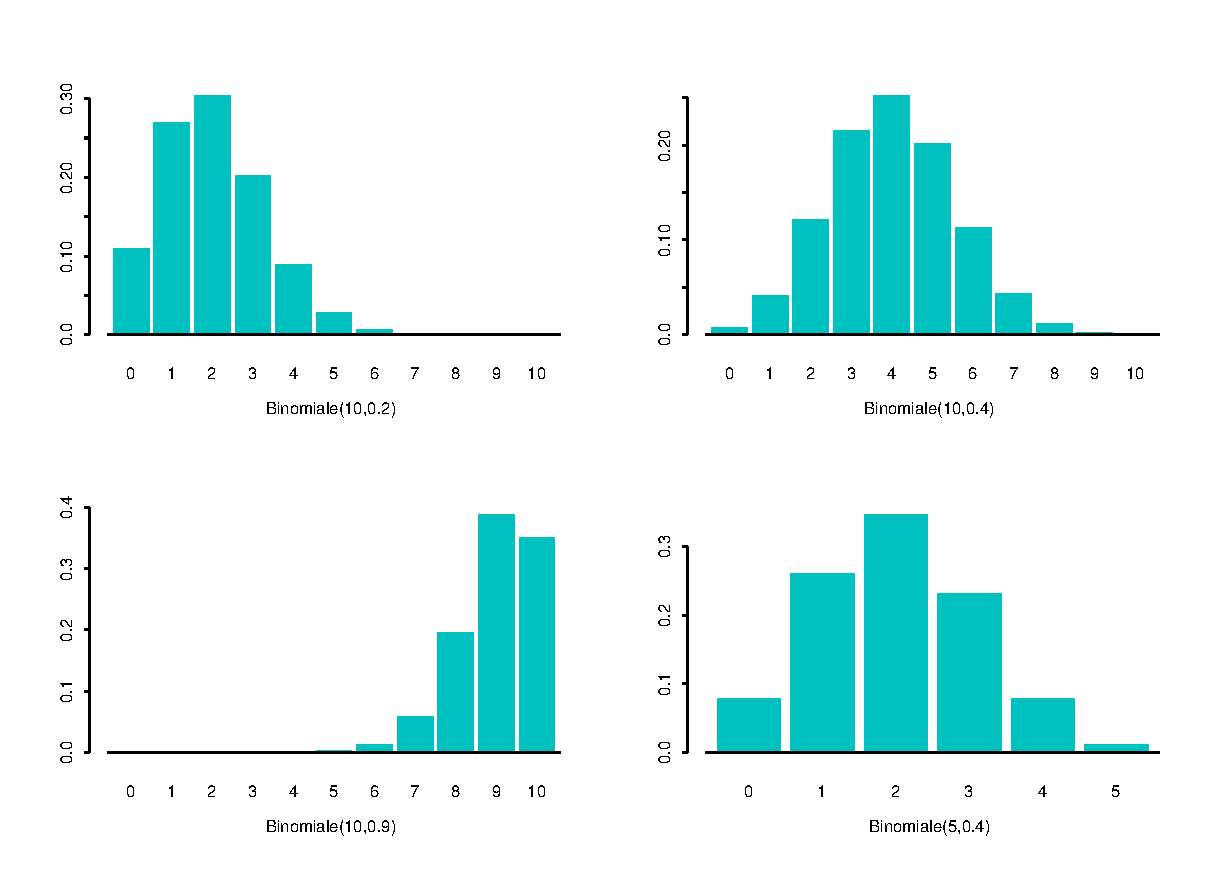
\includegraphics[width=0.75\textwidth,height=0.6\textheight]{img/distbin.pdf}
  \end{figure}
\end{frame}

\begin{frame}{\secname}


\begin{example} [cherry trees]
\begin{footnotesize}

One night a storm washes three cherries ashore on an island. For each cherry, there is a probability $p=0.8$ that its seed will
produce a tree. What is the probability that these three cherries will produce two
trees?

\bigskip

First, we notice that each of these events can be characterised using a \textbf{Bernoulli distribution}.

To this end, consider whether each seed will produce a tree as a sequence of $n=3$
trials. For each cherry:

\begin{itemize}

\item either the cherry produces a tree (Success) or it does not (Failure);
\item the event that a cherry produces a tree is independent from the event
that any of the other two cherries produces a tree.
\item The probability that a cherry produces a tree is the same for all
three cherries
\end{itemize}
\end{footnotesize}
\end{example}

\end{frame}%


\begin{frame}{\secname}%

%\frametitle{Binomial Distribution }

\begin{example}[continued]

\begin{figure}[ptb]\centering
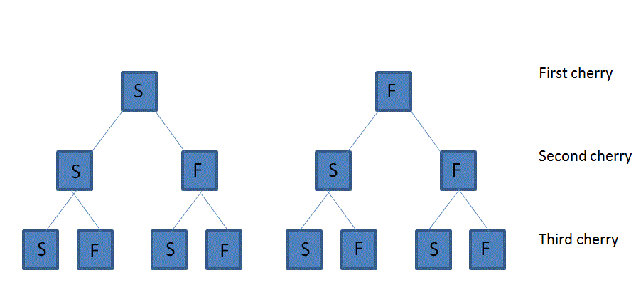
\includegraphics[]{img/BINOMIALpic__1.pdf}
\end{figure}

\end{example}
\end{frame}%

\begin{frame}{\secname}%

%\frametitle{Binomial Distribution}

\begin{example}[continued]
\begin{footnotesize}
\begin{stepitemize}
\item There are $2^{3}=8$ possible outcomes from the $3$ individual trials

\item It does not matter which of the three cherries produce a tree

\item Consider all of the possible sequences of outcomes (S=success,
F=failure)%
\begin{equation*}
\text{SSS,
\color{red}%
SSF,
\color{black}%
\color{red}%
SFS%
\color{black}%
, SFF,
\color{red}%
FSS
\color{black}, FSF, FFS, FFF}
\end{equation*}

\item We are interested in
%TCIMACRO{\TeXButton{red}{\color{red}}}%
%BeginExpansion
\color{red}%
SSF%
%TCIMACRO{\TeXButton{black}{\color{black}}}%
%BeginExpansion
\color{black}%
,
\color{red}%
SFS%
%TCIMACRO{\TeXButton{black}{\color{black}}}%
%BeginExpansion
\color{black}%
%EndExpansion
,
%TCIMACRO{\TeXButton{red}{\color{red}}}%
%BeginExpansion
\color{red}%
%EndExpansion
FSS%
%TCIMACRO{\TeXButton{black}{\color{black}}}%
%BeginExpansion
\color{black}%
%EndExpansion

\item These possible events are \emph{mutually exclusive}, so%
\begin{equation*}
\Pr (\left\{
%TCIMACRO{\TeXButton{red}{\color{red}}}%
%BeginExpansion
\color{red}%
%EndExpansion
SSF%
%TCIMACRO{\TeXButton{black}{\color{black}}}%
%BeginExpansion
\color{black}%
%EndExpansion
\cup
%TCIMACRO{\TeXButton{red}{\color{red}}}%
%BeginExpansion
\color{red}%
%EndExpansion
SFS%
%TCIMACRO{\TeXButton{black}{\color{black}}}%
%BeginExpansion
\color{black}%
%EndExpansion
\cup
%TCIMACRO{\TeXButton{red}{\color{red}}}%
%BeginExpansion
\color{red}%
%EndExpansion
FSS%
%TCIMACRO{\TeXButton{black}{\color{black}}}%
%BeginExpansion
\color{black}%
%EndExpansion
\right\}) =\Pr (\left\{
%TCIMACRO{\TeXButton{red}{\color{red}}}%
%BeginExpansion
\color{red}%
%EndExpansion
SSF%
%TCIMACRO{\TeXButton{black}{\color{black}}}%
%BeginExpansion
\color{black}%
%EndExpansion
\right\}) +\Pr (\left\{
%TCIMACRO{\TeXButton{red}{\color{red}}}%
%BeginExpansion
\color{red}%
%EndExpansion
SFS%
%TCIMACRO{\TeXButton{black}{\color{black}}}%
%BeginExpansion
\color{black}%
%EndExpansion
\right\}) +\Pr (\left\{
%TCIMACRO{\TeXButton{red}{\color{red}}}%
%BeginExpansion
\color{red}%
%EndExpansion
FSS%
%TCIMACRO{\TeXButton{black}{\color{black}}}%
%BeginExpansion
\color{black}%
%EndExpansion
\right\})
\end{equation*}
\end{stepitemize}
\end{footnotesize}
\end{example}
%TCIMACRO{\TeXButton{EndFrame}{\end{frame}}}%
%BeginExpansion
\end{frame}%
%EndExpansion

%TCIMACRO{\TeXButton{BeginFrame}{\begin{frame}{\secname}}}%
%BeginExpansion
\begin{frame}{\secname}%
  %EndExpansion

  %\frametitle{Binomial Distribution}

  \begin{example}[continued]
  \begin{footnotesize}
  The three trials are assumed to be \emph{independent}, so
  each of the three seed events corresponding to two trees growing has
  the same probability%\footnote{Here the symbol ''$\times$" indicates the product}:%
  \begin{eqnarray*}
  \Pr (\left\{
  %TCIMACRO{\TeXButton{red}{\color{red}}}%
  %BeginExpansion
  \color{red}%
  %EndExpansion
  SSF%
  %TCIMACRO{\TeXButton{black}{\color{black}}}%
  %BeginExpansion
  \color{black}%
  %EndExpansion
  \right\})  &=&\Pr (\left\{
  %TCIMACRO{\TeXButton{red}{\color{red}}}%
  %BeginExpansion
  \color{red}%
  %EndExpansion
  S%
  %TCIMACRO{\TeXButton{black}{\color{black}}}%
  %BeginExpansion
  \color{black}%
  %EndExpansion
  \right\}) \cdot \Pr (\left\{
  %TCIMACRO{\TeXButton{red}{\color{red}}}%
  %BeginExpansion
  \color{red}%
  %EndExpansion
  S%
  %TCIMACRO{\TeXButton{black}{\color{black}}}%
  %BeginExpansion
  \color{black}%
  %EndExpansion
  \right\} ) \cdot (\Pr \left\{
  %TCIMACRO{\TeXButton{red}{\color{red}}}%
  %BeginExpansion
  \color{red}%
  %EndExpansion
  F%
  %TCIMACRO{\TeXButton{black}{\color{black}}}%
  %BeginExpansion
  \color{black}%
  %EndExpansion
  \right\}  ) \\
  &=&0.8\cdot 0.8\cdot (1-0.8) \\
  &=&0.8\cdot (1-0.8)\cdot 0.8 =\Pr (\left\{
  %TCIMACRO{\TeXButton{red}{\color{red}}}%
  %BeginExpansion
  \color{red}%
  %EndExpansion
  SFS%
  %TCIMACRO{\TeXButton{black}{\color{black}}}%
  %BeginExpansion
  \color{black}%
  %EndExpansion
  \right\})  \\
  &=&(1-0.8)\cdot 0.8\cdot 0.8= \Pr (\left\{
  %TCIMACRO{\TeXButton{red}{\color{red}}}%
  %BeginExpansion
  \color{red}%
  %EndExpansion
  FSS
  %TCIMACRO{\TeXButton{black}{\color{black}}}%
  %BeginExpansion
  \color{black}%
  %EndExpansion
  \right\} ) \\
  &=&0.128
  \end{eqnarray*}

  So the probability of two trees resulting from the three seeds must be%
  \begin{eqnarray*}
  \Pr (\left\{
  %TCIMACRO{\TeXButton{red}{\color{red}}}%
  %BeginExpansion
  \color{red}%
  %EndExpansion
  SSF%
  %TCIMACRO{\TeXButton{black}{\color{black}}}%
  %BeginExpansion
  \color{black}%
  %EndExpansion
  \cup
  %TCIMACRO{\TeXButton{red}{\color{red}}}%
  %BeginExpansion
  \color{red}%
  %EndExpansion
  SFS%
  %TCIMACRO{\TeXButton{black}{\color{black}}}%
  %BeginExpansion
  \color{black}%
  %EndExpansion
  \cup
  %TCIMACRO{\TeXButton{red}{\color{red}}}%
  %BeginExpansion
  \color{red}%
  %EndExpansion
  FSS%
  %TCIMACRO{\TeXButton{black}{\color{black}}}%
  %BeginExpansion
  \color{black}%
  %EndExpansion
  \right\} ) &=&3\cdot 0.128 \\
  &=&0.384.
  \end{eqnarray*}
  \end{footnotesize}
  \end{example}
\end{frame}



\begin{frame}{\secname}

  \begin{example}
  \begin{footnotesize}
  Finally, we notice that we can obtain the same result (in a more direct way), using the \textbf{binomial probability} for the random variable

  $$X= \text{number of trees that grow from 3 seeds}.$$

  Indeed

  \begin{eqnarray*}
  \Pr (\left\{ X=2\right\})  &=&\frac{3!}{2!\left( 3-2\right) !}\cdot \left(
  0.8\right) ^{2} \cdot \left( 1-0.8\right) ^{3-2} \\
  &=&3 \cdot \left( 0.8\right) ^{2} \cdot \left( 0.2\right)  \\
  &=&0.384.
  \end{eqnarray*}
  \end{footnotesize}
  \end{example}


\end{frame}%

%%%%%%%%%%%%%%%%%%%%%%%%%%%%%%%%%%%%%%%%%%%%%%%%%%%%%%%%%%%%%%%%%%%%%%%%%%%%%%%%
\section{Poisson}
%%%%%%%%%%%%%%%%%%%%%%%%%%%%%%%%%%%%%%%%%%%%%%%%%%%%%%%%%%%%%%%%%%%%%%%%%%%%%%%%

\begin{frame}{\secname}

  %\frametitle{Poisson Distribution}

  \begin{definition}
  Let us consider random variable $X$ which takes values $0,1,2,\dots$, i.e. elements of $\mathbb{N}$.

  $X$ is said to be a Poisson random variable if its probability mass function, with $\lambda >0$ fixed and providing info on the \emph{intensity}, is:
  \begin{equation}
  p(x)=\Pr \left( \{ X = x \}\right) =\frac{\lambda ^{x}e^{-\lambda }}{x!}\text{,\qquad }%
  x=0,1,2,... \label{Eq. Poisson}
  \end{equation}
  and we write $X\sim \mathcal{P}(\lambda)$.
  \end{definition}
  \vspace{0.2cm}
  The Eq. (\ref{Eq. Poisson}) defines a genuine probability mass function, since $p(x) \geq 0$ and
  \bea
  \sum_{x=0}^{\infty} p(x) &=& \sum_{x=0}^{\infty}  \frac{\lambda ^{x}e^{-\lambda }}{x!}  \nn \\
  & = & e^{-\lambda } \sum_{x=0}^{\infty}   \frac{\lambda ^{x}}{x!} \nn \\
  & = & e^{-\lambda } e^{\lambda } = 1 \nn \quad \text{(see Intro Lecture).}
  \eea
\end{frame}%

\begin{frame}{\secname}
  %\frametitle{Poisson Distribution}

  Moreover, for a given value of $\lambda $ also the CDF can be easily defined. E.g.

  \begin{equation*}
  F_X(2)=\Pr \left( \{X\leq 2\}\right) =e^{-\lambda }+\lambda e^{-\lambda }+\frac{\lambda
  ^{2}e^{-\lambda }}{2},
  \end{equation*}

  and the Expected value and Variance for Poisson distribution (see tutorial) can be obtained by ``sum algebra'' (and/or some algebra)

  \begin{eqnarray*}
  E\left[ X\right] &=&\lambda \\
  Var\left( X\right) &=&\lambda.
  \end{eqnarray*}
\end{frame}


\begin{frame}{\secname}
  \begin{figure}[ptb]\centering
  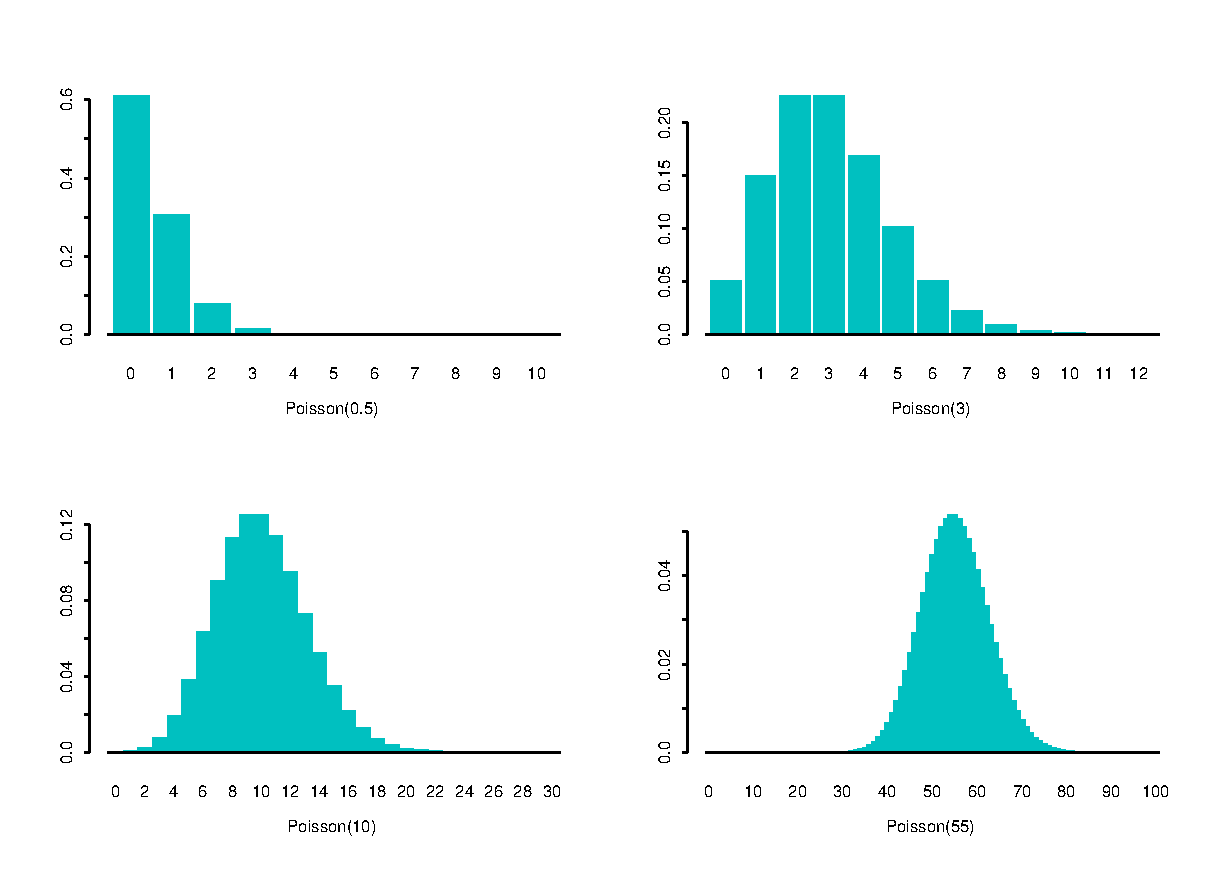
\includegraphics[width=0.75\textwidth]{img/distpois.pdf}
  \end{figure}
\end{frame}


\begin{frame}{\secname}
  \begin{example}
  \begin{footnotesize}
  \emph{The average number of newspapers sold by Alfred is 5 per minute\footnote{This number provides info on the intensity
  at which a random phenomenon occurs.}. What is the probability that Alfred will sell at least 1 newspaper in a minute?} \medskip
  \pause

  To answer, let $X$ be the $\#$ of newspapers sold by Alfred in a minute. We have
  $$
  X \sim \mathcal{P}(\lambda)
  $$
  with $\lambda = 5$, so
  \begin{eqnarray*}
  P(X \geq 1) & = & 1- P(\{X=0\}) \\
  & = & 1 - \exp^{-5} \frac{5^0}{0!} \\
  %& = & 1-\exp^{-5} \\
  & \approx & 1- 0.0067 \approx 99.33\%.
  \end{eqnarray*}
  How about $P(X \geq 2)$? Is it $P(X \geq 2) \geq P(X \geq 1)$ or not? Answer the question...
  \end{footnotesize}
  \end{example}
\end{frame}

\begin{frame}{\secname}
  \begin{example}
  \begin{footnotesize}
  A telephone switchboard handles 300 calls, on the average, during one hour. The board
  can make maximum 10 connections per minute. Use the Poisson
  distribution to evaluate the probability that the board will be overtaxed during a given minute.

  \medskip

  To answer, let us set  $\lambda = 300$ per hour, which is equivalent to 5 calls per minute. Noe let us define
  $$
  X = \text{\# of connections in a minute}
  $$
  and by assumption we have $X \sim \mathcal{P}(\lambda)$. Thus,
  \bea
  P[\text{overtaxed}] &=& P(\{X > 10\}) \nn \\
  &=& 1 \quad - \underbrace{P(\{X \leq 10\})}_{\text{using $\lambda=5$,  minute base}} \nn \\
  &\approx& 0.0137. \nn
  \eea
  \end{footnotesize}
  \end{example}
\end{frame}


\begin{frame}{\secname}
\framesubtitle{Links to the Binomial Distribution}
  \begin{remark}
  Let us consider $X \sim \mathcal{B}(n,p)$, \textcolor{red} {where $n$ is large, $p$ is small, and the product $np$ is noticeable}. Setting, $\lambda=np$, we
  then have that, for the Binomial probability as in Eq.(\ref{Eq: Binom}), it is a good approximation to write:
  $$
  p(k) = P(\{X=k\}) \approx \frac{\lambda^k}{k!} e^{-\lambda}.
  $$
  \end{remark}
  \pause
  \begin{proof}
  \begin{footnotesize}
  To see this, remember that
  $$
  \lim_{n\rightarrow\infty} \left( 1- \frac{\lambda}{n} \right)^n = e^{-\lambda}.
  $$
  Then, let us consider that in our setting, we have $p=\lambda/n$. From the formula of the binomial probability mass function we have:
  $$
  p(0) = (1-p)^{n}=\left( 1- \frac{\lambda}{n} \right)^{n} \approx e^{-\lambda}, \quad \text{\ as \ \ } n\rightarrow\infty.
  $$
  \end{footnotesize}
  \end{proof}
\end{frame}

\begin{frame}{\secname}%
\framesubtitle{Links to the Binomial Distribution}
  \begin{proof}
  \begin{footnotesize}
  Moreover, it is easily found that

  \bea
  \frac{p(k)}{p(k-1)} &=& \frac{np-(k-1)p}{k(1-p)} \approx \frac{\lambda}{k}, \quad \text{\ as \ \ } n\rightarrow\infty. \nn
  \eea
  Therefore, we have
  \bea
  p(1) &\approx& \frac{\lambda}{1!}p(0) \approx \lambda e^{-\lambda} \nn \\
  p(2) &\approx& \frac{\lambda}{2!}p(1) \approx \frac{\lambda^2}{2} e^{-\lambda} \nn \\
  \dotsm & \dotsm &  \dotsm  \nn \\
  p(k) &\approx& \frac{\lambda}{k!}p(k-1) \approx \underbrace{\frac{\lambda^k}{k!} e^{-\lambda}}_{\text{\ see \ \ Eq. (\ref{Eq. Poisson})  }} \nn
  \eea

  thus, we remark that $p(k)$ can be approximated by the probability mass function of a Poisson --- which is easier to evaluate.
  \end{footnotesize}
  \end{proof}
\end{frame}

\begin{frame}{\secname}%
%EndExpansion

%\frametitle{Poisson Distribution: example}
\begin{example}[two-fold use of Poisson]
\begin{footnotesize}
\emph{Suppose a certain high-speed printer makes errors at random on printed paper\footnote{This exercise is related to Ex 2 of PS6. The calculation is similar but not identical: notice the difference between the size of $p$ in this example and in the tutorial.}.

Assuming that the Poisson
distribution with parameter $\lambda = 4$ is appropriate to model the number of errors per page (say, $X$), what is the probability that in a book containing 300 pages (produced by the printer) at least 7 will have no errors?}

\medskip

Let $X$ denote the number of errors per page, so that
$$
p(x) = \exp(-4)\frac{4^x}{x!}, \quad \text{for} \quad x = 0,1,2,....
$$
The probability of any page to be error free is then
$$p(0) = \exp(-4)\frac{4^0}{0!} = \exp(-4)\approx 0.018.$$
\end{footnotesize}
\end{example}
\end{frame}%

\begin{frame}{\secname}%

  \begin{example}[cont'd]
  \begin{footnotesize}
  Having no errors on a page is a success, and there are 300 independent pages. Hence, let us define
  $$
  Y = \text{the number of pages without any errors}.
  $$

  $Y$ is binomially distributed with parameters $n = 300$
  and $p = 0.018$, namely
  $$Y\sim \mathcal{B}(n,p).$$


  But here we have
  \begin{center}
  $n$ large, $p$ small, and $n p = 5.4$
  \end{center}
  thus, we can compute $P(\{Y \geq 7\})$  using either the exact Binomial or its Poisson approximation. So
  \begin{itemize}
  \item using $\mathcal{B}(300,0.018)$, we get: $P(\{Y \geq 7\}) \approx  0.297$ \\ \vspace{0.1cm}

  \item using $\mathcal{P}(5.4)$, we get $P(\{Y \geq 7\})  \approx  0.298.$
  \end{itemize}
  %The two outcomes differ at the 3rd digits after the comma.
  \end{footnotesize}
  \end{example}
\end{frame}%

%%%%%%%%%%%%%%%%%%%%%%%%%%%%%%%%%%%%%%%%%%%%%%%%%%%%%%%%%%%%%%%%%%%%%%%%%%%%%%%%
\section{Hypergeometric}
%%%%%%%%%%%%%%%%%%%%%%%%%%%%%%%%%%%%%%%%%%%%%%%%%%%%%%%%%%%%%%%%%%%%%%%%%%%%%%%%

\begin{frame}{\secname}
  %\frametitle{The Hypergeometric Distribution}

  \begin{definition}
  Let us consider a random experiment consisting of a series of $n$ trials,
  having the following properties

  \begin{stepenumerate}
  \item Only two mutually exclusive outcomes are possible in each trial:
  success ($S$) and failure ($F$)

  \item The population has $N$ elements with $k$ Successes $S$ and $N-k$ Failures $F$

  \item Sampling from the population is done \textbf{without} replacement (so
  that the \textbf{trials are not independent}).
  \end{stepenumerate}

  The random variable
  $$
  X= \text{number of successes in $n$ such trials}
  $$
  has an hypergeometric distribution and \dots
  \end{definition}
\end{frame}

\begin{frame}{\secname}
  %\frametitle{The Hypergeometric Distribution}

  \begin{definition}[cont'd]
  ... the probability that $X=x$ is
  \begin{equation*}
  \Pr (\left\{ X=x\right\}) =\frac{\left(
  \begin{array}{c}
  k \\
  x%
  \end{array}%
  \right) \left(
  \begin{array}{c}
  N-k \\
  n-x%
  \end{array}%
  \right) }{\left(
  \begin{array}{c}
  N \\
  n%
  \end{array}%
  \right) }.
  \end{equation*}
  \end{definition}

  Moreover,
  \begin{eqnarray*}
  E\left[ X\right] &=&\frac{nk}{N} \\
  Var\left( X\right) &=&\frac{nk\left( N-k\right) \left( N-n\right) }{%
  N^{2}\left( N-1\right) }
  \end{eqnarray*}
\end{frame}

\begin{frame}{\secname}
  %\frametitle{Hypergeometric Distribution Example}

  \begin{example}[Psychological experiment]
  A group of 8 students includes 5 women and 3 men: 3 students are randomly chosen to participate in a psychological
  experiment. What is the probability that \emph{exactly} 2 women will be included
  in the sample?%
  %TCIMACRO{%
  %\FRAME{ftbpF}{2.1966in}{2.207in}{0pt}{}{}{urnpic.gif}{%
  %\special{language "Scientific Word";type "GRAPHIC";maintain-aspect-ratio TRUE;display "USEDEF";valid_file "F";width 2.1966in;height 2.207in;depth 0pt;original-width 6.9168in;original-height 6.9479in;cropleft "0";croptop "1";cropright "1";cropbottom "0";filename '../URNpic.GIF';file-properties "XNPEU";}}}%
  %BeginExpansion
  \begin{figure}[ptb]\centering
  %\includegraphics[natheight=6.9479in, natwidth=6.9168in, height=2.207in, width=2.1966in]
  %{//ad.monash.edu/home/User063/scipione/Documents/CF2015/teaching/ETC2520/NEW_ETC25250/lecture6_2015/graphics/img/URNpic__2.pdf}%
  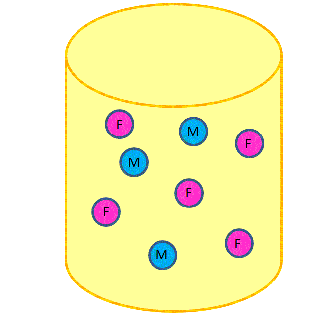
\includegraphics[width=0.4\textwidth]{img/URNpic_2.pdf}
  \end{figure}
  \end{example}
\end{frame}%


\begin{frame}{\secname}
\framesubtitle{Example}
  %\frametitle{Hypergeometric Distribution Example}
  \begin{example}[cont'd]
  Consider each of the three participants being selected as a separate
  trial $\Rightarrow $ there are $n=3$ trials. Consider a woman being selected in a trial as a `success'
  \\
  Then here $N=8$, $k=5$, $n=3$, and $x=2$, so that%
  \begin{eqnarray*}
  \Pr (\left\{ X=2\right\})  &=&\frac{\left(
  \begin{array}{c}
  5 \\
  2%
  \end{array}%
  \right) \left(
  \begin{array}{c}
  8-5 \\
  3-2%
  \end{array}%
  \right) }{\left(
  \begin{array}{c}
  8 \\
  3%
  \end{array}%
  \right) } \\
  && \\
  &=&\frac{\frac{5!}{2!3!}\frac{3!}{1!2!}}{\frac{8!}{5!3!}} \\
  && \\
  &=&0.53571
  \end{eqnarray*}
  \end{example}
\end{frame}


%%%%%%%%%%%%%%%%%%%%%%%%%%%%%%%%%%%%%%%%%%%%%%%%%%%%%%%%%%%%%%%%%%%%%%%%%%%%%%%%
\section{Negative Binomial}
%%%%%%%%%%%%%%%%%%%%%%%%%%%%%%%%%%%%%%%%%%%%%%%%%%%%%%%%%%%%%%%%%%%%%%%%%%%%%%%%


\begin{frame}{\secname}%
  \begin{definition}

  Let us consider a random experiment consisting of a series of trials, having
  the following properties \medskip

  \begin{stepenumerate}
  \item Only two mutually exclusive outcomes are possible in each trial:
  `success' (S) and `failure' (F)
  \medskip
  \item The outcomes in the series of trials constitute \emph{independent
  events}
  \medskip
  \item The probability of success $p$ in each trial is \emph{constant }from
  trial to trial
  \end{stepenumerate}
  \medskip
  What is the probability of having exactly $y$ F's before the $r^{th}$
  S? \\ \medskip

  Equivalently: What is the probability that in a sequence of $y+r$ (Bernoulli) trials the last trial yields the
  $r^{th}$ S?
  \end{definition}
\end{frame}

\begin{frame}{\secname}
  \begin{definition}
  Let
  $$X= \text{the total number of trials required until a total of $r$ successes is accumulated}.$$
  Then $X$ is said to be a Negative Binomial random variable and its probability mass function
  $\Pr (\left\{ X=n\right\})$ equals the probability of $r-1$ `successes' in the first $n-1$ trials, times the probability of a `success' on
  the last trial. These probabilities are given by%
  \begin{equation*}
  \Pr (\left\{ X=n\right\}) =\left(
  \begin{array}{c}
  n-1 \\
  r-1%
  \end{array}
  \right) p^{r}\left( 1-p\right) ^{n-r}\quad \text{ for }n=r,r+1,...
  \end{equation*}
  \end{definition}

  The mean and variance for $X$ are, respectively,%
  \begin{eqnarray*}
  E\left[ X\right] &=&\frac{r}{p} \\
  Var\left( X\right) &=&\frac{r\left( 1-p\right) }{p^{2}}
  \end{eqnarray*}
\end{frame}%

\begin{frame}{\secname}
  \framesubtitle{Example}

  \begin{example}[marketing research]
  \begin{stepitemize}

  \item A marketing researcher wants to find 5 people to join her focus group

  \item Let $p$ denote the probability that a randomly selected individual
  agrees to participate in the focus group

  \item If $p=0.2$, what is the probability that the researcher must ask 15
  individuals before 5 are found who agree to participate?

  %\item That is, what is the probability that 10 people will decline the
  %request to participate before a 5$^{th}$ person agrees?

  \item In this case, $p=0.2$, $r=5$, $n=15$:  we are looking for $\Pr (\left\{
  X=15\right\}).$ By the negative binomial formula we have

  \begin{eqnarray*}
  \Pr (\left\{ X=15\right\}) &=&\left(
  \begin{array}{c}
  14 \\
  4%
  \end{array}%
  \right) \left( 0.2\right) ^{5}\left( 0.8\right) ^{10} \\
  &=&0.034
  \end{eqnarray*}
  \end{stepitemize}
  \end{example}
\end{frame}

%%%%%%%%%%%%%%%%%%%%%%%%%%%%%%%%%%%%%%%%%%%%%%%%%%%%%%%%%%%%%%%%%%%%%%%%%%%%%%%%
\section{Geometric}
%%%%%%%%%%%%%%%%%%%%%%%%%%%%%%%%%%%%%%%%%%%%%%%%%%%%%%%%%%%%%%%%%%%%%%%%%%%%%%%%


\begin{frame}{\secname}
  \begin{definition}[a special case]

  When $r=1$, the negative binomial distribution is equivalent to the
  \textbf{Geometric distribution} --- see the example in the previous lecture. \\
  \medskip
  In this case, probabilities are given by%
  \begin{equation*}
  \Pr (\left\{ X=n\right\}) =p\left( 1-p\right) ^{n-1}\text{, for }n=1,2,...
  \end{equation*}
  \end{definition}

  The corresponding mean and variance for $X$ are, respectively,%
  \begin{eqnarray*}
  E\left[ X\right] &=&\frac{ 1 }{p} \\
  Var\left( X\right) &=&\frac{\left( 1-p\right) }{p^{2}}
  \end{eqnarray*}
\end{frame}

\begin{frame}{\secname}
  \begin{small}

  \begin{example}[failure of a machine]
  \begin{footnotesize}
  Items are produced by a machine having a 3\% defective rate.
  \begin{itemize}
  \item What is the probability that the first defective occurs in the fifth item inspected? \\
  \bea
  P(\{X	=	5\})	&=&	P (\text{first	4	non-defective}) P (\text{5th defective}) \nn \\
  &=& (0.97)^4(0.03) \approx 0.026 \nn
  \eea
  \item What is the probability that the first defective occurs in the first five inspections?
  \bea
  P(\{X	\leq 5	\}) = P(\{X	< 6	\})	&=&	 P (\{X=1\})+ ... + P(\{X=5\}) \nn \\
  &=& 1- P(\text{first 5 non-defective}) = 0.1412.  \nn %\\
  %&=& 1- (0.97)^5 \approx 0.1412 \nn
  \eea
  \end{itemize}
  \end{footnotesize}
  \end{example}

  More generally, for a geometric random variable we have:
  $$
  P(\{X \geq k \}) = (1-p)^{k-1}.
  $$
  Thus, in the example we have $P( \{X	\geq 6	\}) = (1-0.03)^{6-1}\approx 0.8587$
  \bea
  P(\{X	\leq 5	\}) = 1-P( \{X	\geq 6	\}) \approx 1- 0.8587 \approx 0.1412. \nn
  \eea
  \end{small}
\end{frame}

\begin{frame}{Wrap-up}
  It is important to keep in mind and review:
  \bigskip
  \begin{itemize}
  \item The expressions of the PMF's of the different functions.
  \medskip
  \item Their case uses (When to use Bernoulli, Binomial, Poisson, \dots)
  \medskip
  \item The link between Poisson and Binomial, as it simplifies the computations.
  \end{itemize}
\end{frame}


\begin{frame}
  \begin{center}
  \Large{Thank You for your Attention!}

  \bigskip
  \pause


  \Large{``See you'' Next Week}
  \end{center}
\end{frame}

\end{document}
